% --------------------
\mysec{Kongruenzsätze}
% --------------------
\formnum \textbf{SSS:} Zwei Dreiecke, die in ihren drei Seitenlängen
übereinstimmen, sind kongruent.\medskip\par
\formnum \textbf{SWS:} Zwei Dreiecke, die in zwei Seitenlängen und in
dem eingeschlossenen Winkel übereinstimmen, sind kongruent.\medskip\par
\formnum \textbf{WSW:} Zwei Dreiecke, die in einer Seitenlänge und in
den dieser Seite anliegenden Winkeln übereinstimmen, sind kongruent.\medskip\par
\formnum \textbf{SsW:} Zwei Dreiecke, die in zwei Seitenlängen und in
jenem Winkel übereinstimmen, der der längeren Seite gegenüberliegt,
sind kongruent.\medskip\par
\begin{center}
  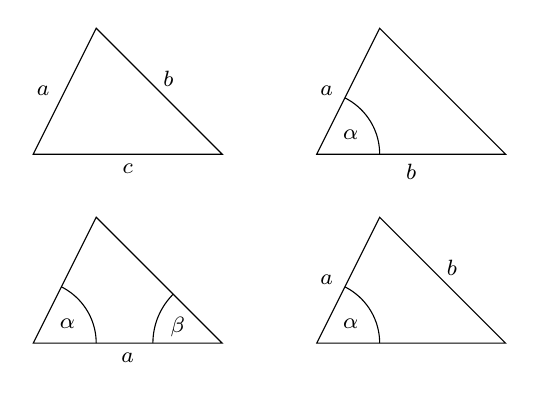
\begin{tikzpicture}[scale=0.8]
    \begin{scope}
      \draw (0, 0) -- (3, 0) -- (1, 2) -- cycle;
      \path (0, 0) -- node[below]{{\footnotesize$c$}}
            (3, 0) -- node[above right=-2pt]{{\footnotesize$b$}}
            (1, 2) -- node[left=2pt]{{\footnotesize$a$}}
            (0, 0);
    \end{scope}
    \begin{scope}[xshift=4.5cm]
      \draw (0, 0) -- (3, 0) -- (1, 2) -- cycle;
      \path (0, 0) -- node[below]{{\footnotesize$b$}}
            (3, 0) --
            (1, 2) -- node[left=2pt]{{\footnotesize$a$}}
            (0, 0);
      \begin{scope}
        \clip (0, 0) -- (3, 0) -- (1, 2) -- cycle;
        \draw (0, 0) circle (1cm);
        \node[shift=(30:5mm)] at (0, 0) {{\footnotesize$\alpha$}};
      \end{scope}
    \end{scope}
    \begin{scope}[yshift=-3cm]
      \draw (0, 0) -- node[below]{{\footnotesize$a$}}
            (3, 0) --
            (1, 2) -- cycle;
      \begin{scope}
        \clip (0, 0) -- (3, 0) -- (1, 2) -- cycle;
        \draw (0, 0) circle (1cm);
        \node[shift=(30:5mm)] at (0, 0) {{\footnotesize$\alpha$}};
      \end{scope}
      \begin{scope}
        \clip (0, 0) -- (3, 0) -- (1, 2) -- cycle;
        \draw (3, 0) circle (1.1cm);
        \node[shift=(160:6mm)] at (3, 0) {{\footnotesize$\beta$}};
      \end{scope}
    \end{scope}
    \begin{scope}[xshift=4.5cm, yshift=-3cm]
      \draw (0, 0) -- (3, 0) -- (1, 2) -- cycle;
      \path (0, 0) --
            (3, 0) -- node[above right=-2pt]{{\footnotesize$b$}}
            (1, 2) -- node[left=2pt]{{\footnotesize$a$}}
            (0, 0);
      \begin{scope}
        \clip (0, 0) -- (3, 0) -- (1, 2) -- cycle;
        \draw (0, 0) circle (1cm);
        \node[shift=(30:5mm)] at (0, 0) {{\footnotesize$\alpha$}};
      \end{scope}
    \end{scope}
  \end{tikzpicture}
\end{center}

